\documentclass[border=3pt]{standalone}
\usepackage{tikz}
\usetikzlibrary{calc}
\begin{document}
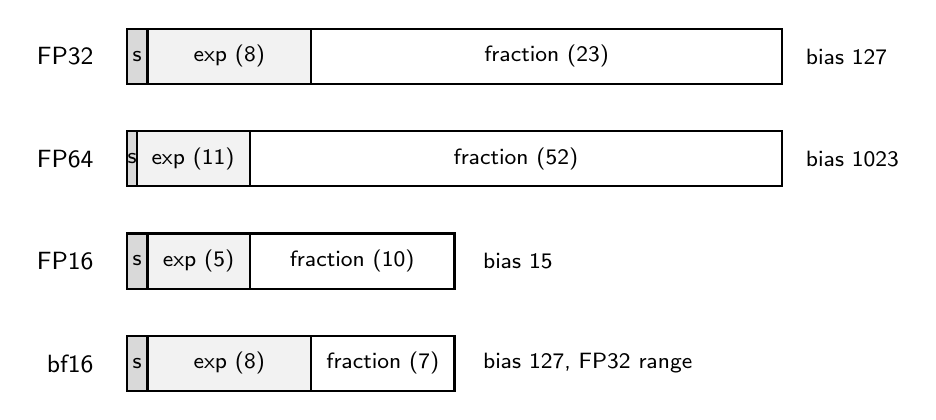
\begin{tikzpicture}[font=\sffamily\small, x=1mm, y=1mm]
  % helper lengths: draw each format as sign|exp|frac boxes, width proportional
  % FP32: 1 | 8 | 23  (scale 2.6mm/bit)
  \begin{scope}[shift={(0,0)}]
    \node[anchor=east] at (-3,3.5) {FP32};
    \draw[thick, fill=black!15] (0,0) rectangle (2.6,7);
    \draw[thick, fill=black!5]  (2.6,0) rectangle (23.4,7);
    \draw[thick] (23.4,0) rectangle (83.2,7);
    \node at (1.3,3.5) {\footnotesize s};
    \node at (13,3.5) {\footnotesize exp (8)};
    \node at (53.3,3.5) {\footnotesize fraction (23)};
    \node[anchor=west, font=\sffamily\footnotesize] at (85,3.5) {bias 127};
  \end{scope}
  % FP64: 1 | 11 | 52 (scale 1.3mm/bit)
  \begin{scope}[shift={(0,-13)}]
    \node[anchor=east] at (-3,3.5) {FP64};
    \draw[thick, fill=black!15] (0,0) rectangle (1.3,7);
    \draw[thick, fill=black!5]  (1.3,0) rectangle (15.6,7);
    \draw[thick] (15.6,0) rectangle (83.2,7);
    \node at (0.65,3.5) {\footnotesize s};
    \node at (8.4,3.5) {\footnotesize exp (11)};
    \node at (49.4,3.5) {\footnotesize fraction (52)};
    \node[anchor=west, font=\sffamily\footnotesize] at (85,3.5) {bias 1023};
  \end{scope}
  % FP16: 1 | 5 | 10 (scale 2.6mm/bit)
  \begin{scope}[shift={(0,-26)}]
    \node[anchor=east] at (-3,3.5) {FP16};
    \draw[thick, fill=black!15] (0,0) rectangle (2.6,7);
    \draw[thick, fill=black!5]  (2.6,0) rectangle (15.6,7);
    \draw[thick] (15.6,0) rectangle (41.6,7);
    \node at (1.3,3.5) {\footnotesize s};
    \node at (9.1,3.5) {\footnotesize exp (5)};
    \node at (28.6,3.5) {\footnotesize fraction (10)};
    \node[anchor=west, font=\sffamily\footnotesize] at (44,3.5) {bias 15};
  \end{scope}
  % bfloat16: 1 | 8 | 7 (scale 2.6mm/bit)
  \begin{scope}[shift={(0,-39)}]
    \node[anchor=east] at (-3,3.5) {bf16};
    \draw[thick, fill=black!15] (0,0) rectangle (2.6,7);
    \draw[thick, fill=black!5]  (2.6,0) rectangle (23.4,7);
    \draw[thick] (23.4,0) rectangle (41.6,7);
    \node at (1.3,3.5) {\footnotesize s};
    \node at (13,3.5) {\footnotesize exp (8)};
    \node at (32.5,3.5) {\footnotesize fraction (7)};
    \node[anchor=west, font=\sffamily\footnotesize] at (44,3.5) {bias 127, FP32 range};
  \end{scope}
\end{tikzpicture}
\end{document}
